\section{METHODOLOGY}
\label{sec:methodology}

\begin{figure*}[t]
\centering
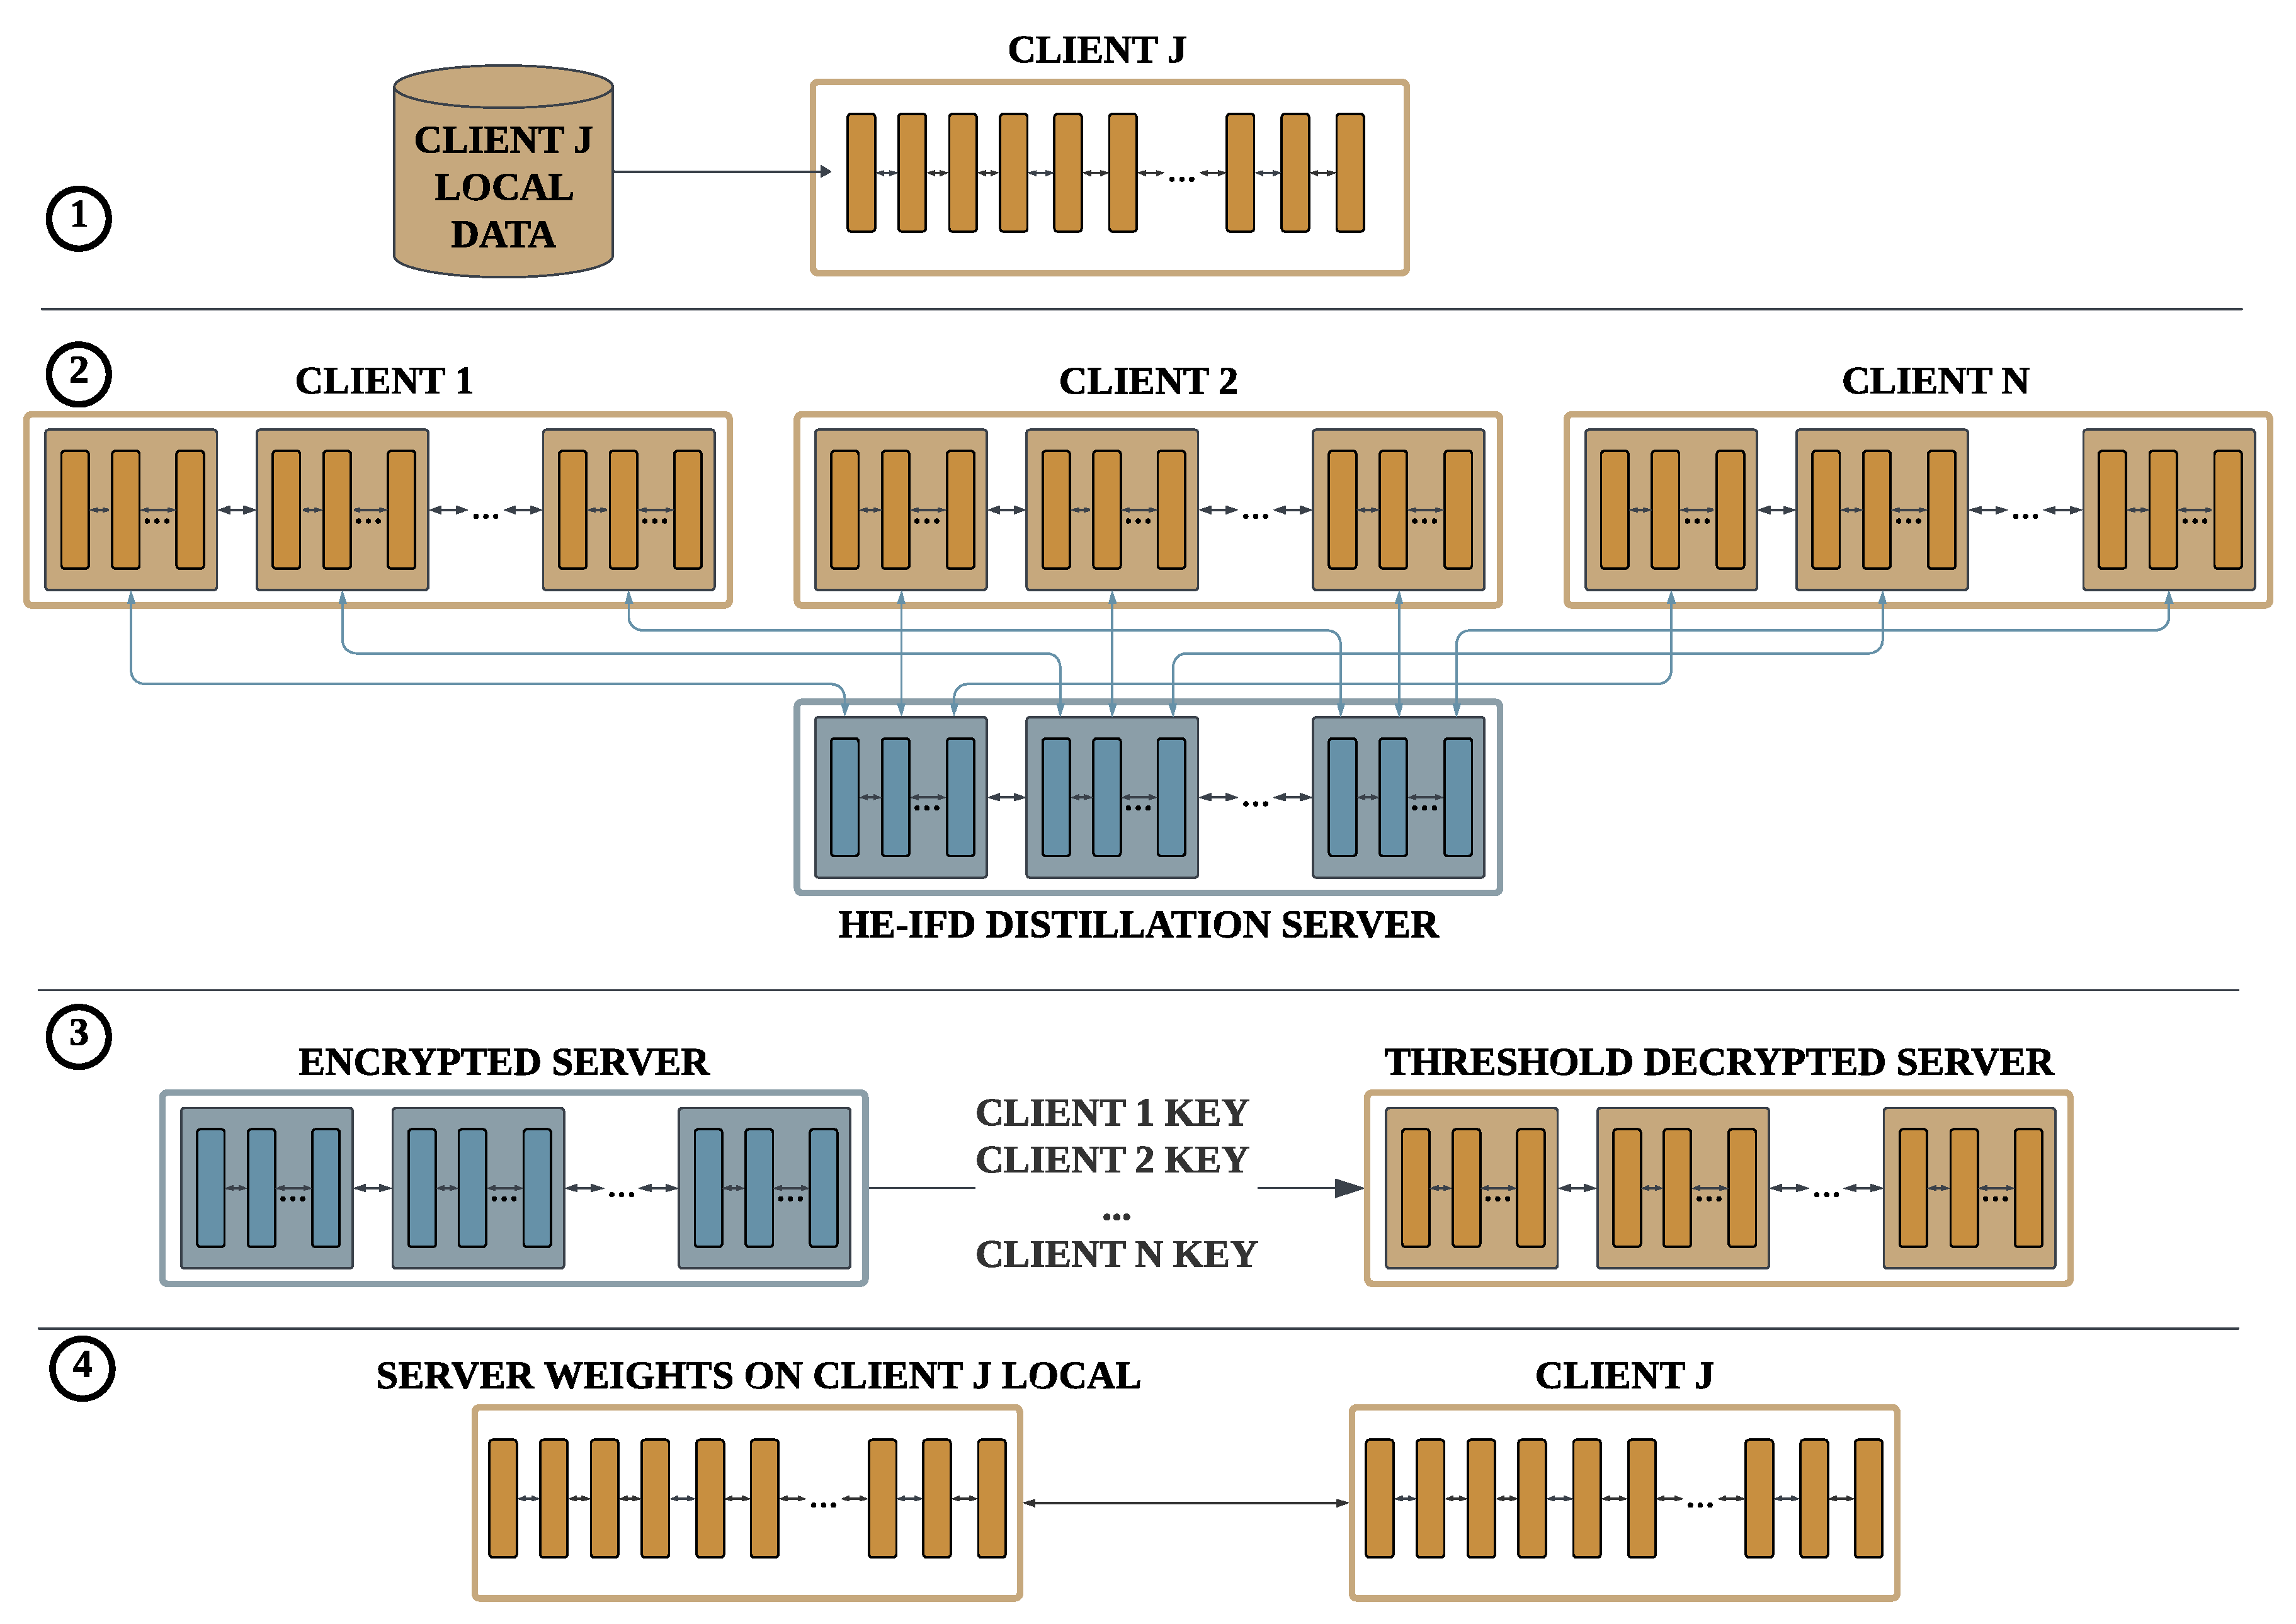
\includegraphics[width=0.87\textwidth]{figures/HE-IFD_sysFigure.pdf}
\caption{Overview of HE-IFD. \textcircled{1}~\textbf{Client-side training.} Each client independently trains a teacher model on its own private dataset. No data leaves the client device. \textcircled{2}~\textbf{Encrypted upload and server distillation.} Every client extracts intermediate feature representations at each block boundary of its teacher, normalises them per channel, encrypts them under the CKKS homomorphic encryption scheme, and uploads the ciphertexts to the server in a single communication round. The server pools encrypted features from all clients and trains a student model block by block, operating entirely on ciphertexts. The server never observes any plaintext data, weights, or intermediate values. \textcircled{3}~\textbf{Threshold decryption.} The server distributes the encrypted student model to all clients. Each client applies its secret key share locally to decrypt the model on its own device. No single client can decrypt alone, and the server never sees plaintext weights. \textcircled{4}~\textbf{Local model assembly.} Each client holds the decrypted student model in plaintext and may optionally fine-tune it on local data to adapt to its own distribution, with no further communication required.}
\label{fig:sys_figure}
\end{figure*}

\subsection{HE-IFD: One-Shot Distillation Framework}
\label{sec:framework}

This section presents the HE-IFD protocol in full generality. The framework applies to any architecture that admits a block decomposition with HE-compatible operations; architecture-specific instantiations are deferred to Section~\ref{sec:architecture}.

% \subsubsection{System Model and Threat Model}
% \label{sec:system_model}

\par\noindent\textbf{System Model.} We consider a cross-silo federated learning setting with $N$ clients and a central server. Each client $i$ holds a private dataset $\mathcal{D}_i$ that is never shared or transmitted. Clients wish to collaboratively train a shared student model by transferring knowledge from their locally trained teacher models to the server, without exposing their private data, including raw training data and any intermediate representations. Communication between clients and the server is restricted to a single round: each client sends a set of encrypted messages derived from its local data and model, after which the server performs all remaining computation independently with no further client interaction. An optional release phase at the end allows clients to collectively obtain the trained model.

\par\noindent\textbf{Threat Model.} We assume a semi-honest (honest-but-curious) server that follows the protocol faithfully but may attempt to infer private information from everything it observes. The adversary's goal is to infer information about a client's private dataset $\mathcal{D}_i$ or the client's local model, including individual samples, label distributions, or model weights, from the messages it receives during training. We further assume that the server may collude with up to $N-1$ clients; privacy of the remaining honest client's input is guaranteed by the threshold structure of the multiparty CKKS scheme described in Section~\ref{sec:phase3}, which requires the joint participation of all $N$ clients to decrypt any ciphertext.

Given this system and threat model, sending plaintext teacher outputs to the server is insufficient. Because, as discussed in Section~\ref{sec:bg_server_inference}, even a single round of plaintext knowledge transfer exposes clients to inference and inversion attacks. We therefore instantiate the knowledge transfer channel using the multiparty CKKS HE scheme~\cite{cheon2017ckks, mouchet2021multiparty} — the same construction implemented in Lattigo~\cite{lattigo} — which lets the server perform all distillation computation directly on ciphertexts under a public key whose corresponding secret key is held in shares across the $N$ clients.

% Under the IND-CPA security of CKKS, the server's entire view during training (encrypted feature pairs, intermediate activations, loss values, gradients, and student weights) is computationally indistinguishable from random. The server operates purely as a blind compute delegate and learns nothing about any client's private data. For additional protection, clients may add calibrated differential privacy noise before encryption, achieving $(\epsilon, \delta)$-differential privacy for the released model; this is optional since the cryptographic guarantee already prevents the server from inspecting any individual contribution during training.


% \subsubsection{Overview of HE-IFD}
% \label{sec:overview}

\par\noindent\textbf{Overview of HE-IFD.} HE-IFD proceeds in four phases, illustrated in Figure~\ref{fig:sys_figure} and formalised in Algorithm~\ref{alg:heifd}. In Phase~1, each client independently trains a teacher model on its private data. In Phase~2, clients extract intermediate features at each block boundary of the teacher, encrypt them under CKKS, and upload to the server in a single communication round, which is the only client-to-server interaction in the entire protocol. The server then trains an HE-compatible student model block by block on the pooled encrypted features. In Phase~3, clients collaboratively perform threshold decryption to obtain the trained student in plaintext. In Phase~4, each client receives the decrypted model (via joint threshold decryption) and may fine-tune it on local data to adapt to its own distribution.

The server never sees any plaintext data, model weights, or intermediate computations. All training happens on encrypted ciphertexts. Each block is trained independently with fresh ciphertexts, so multiplicative levels do not accumulate across blocks.


\begin{algorithm}[t!]
\small
\caption{HE-IFD: HE-Based Intermediate Feature Distillation}
\label{alg:heifd}
\begin{algorithmic}[1]
\REQUIRE $N$ clients with private datasets $\mathcal{D}_1, \ldots, \mathcal{D}_N$; student architecture $S$ with $K{+}1$ blocks
\ENSURE Trained student model $S$

\STATE \textbf{--- Phase 1: Client-Side Training (parallel, local) ---}
\FOR{each client $i = 1, \ldots, N$ \textbf{in parallel}}
    \STATE Train teacher $T_i$ on $\mathcal{D}_i$ via standard SGD
\ENDFOR

\STATE
\STATE \textbf{--- Phase 2: Encrypted Upload + Server Distillation ---}
\FOR{each client $i = 1, \ldots, N$ \textbf{in parallel}}
    \FOR{each block $k = 0, \ldots, K$}
        \STATE Extract feature pairs $(\mathbf{x}_k^{(i,j)}, \mathbf{y}_k^{(i,j)})$ by running $T_i$ on $\mathcal{D}_i$
        \STATE Normalise per channel: $\tilde{\mathbf{y}}_k \leftarrow (\mathbf{y}_k - \mu) / \sigma$ \hfill\COMMENT{Eq.~\ref{eq:client_norm}}
    \ENDFOR
    \STATE Encrypt all pairs under CKKS; upload $\{\enc{\mathbf{x}_k}, \enc{\tilde{\mathbf{y}}_k}\}$ to server \hfill\COMMENT{one-shot}
\ENDFOR

\STATE
\STATE \textit{Server-side (all computation on encrypted data):}
\STATE Initialise student $S$ with near-linear polynomial activations
\FOR{block $k = 0, \ldots, K$}
    \STATE Pool encrypted pairs from all $N$ clients for block $k$; shuffle
    \STATE Set depth-dependent hyperparameters: $\lambda_k, \eta_k$ \hfill\COMMENT{deeper blocks: stronger reg., lower LR}
    \FOR{epoch $= 1, \ldots, E$}
        \FOR{each mini-batch $(\enc{\mathbf{x}}, \enc{\tilde{\mathbf{y}}_k})$}
            \STATE $\hat{\mathbf{y}} \leftarrow S_{\text{block}[k]}(\enc{\mathbf{x}})$ \hfill\COMMENT{encrypted forward pass}
            \STATE $\mathcal{L} \leftarrow \mathcal{L}_{\text{MagReg}}(\hat{\mathbf{y}}, \enc{\tilde{\mathbf{y}}_k})$ \hfill\COMMENT{Eq.~\ref{eq:magreg}}
            \STATE Update $S_{\text{block}[k]}$ via encrypted gradient descent
        \ENDFOR
    \ENDFOR
    \STATE Freeze $S_{\text{block}[k]}$; initialise bridge $\mathbf{b}_k$ from feature statistics
\ENDFOR
\STATE Refine blocks sequentially with bridges on uploaded features ($R$ rounds)

\STATE
\STATE \textbf{--- Phase 3: Threshold Decryption ---}
\STATE All $N$ clients contribute key shares $\rightarrow$ decrypt $S$ to plaintext

\STATE
\STATE \textbf{--- Phase 4: Client-Side Model Assembly ---}
\FOR{each client $i = 1, \ldots, N$}
    \STATE Receive decrypted student $S$
    \STATE (Optional) Fine-tune $S$ on local data $\mathcal{D}_i$ with cross-entropy loss
\ENDFOR
\end{algorithmic}
\end{algorithm}

\subsubsection{Phase~1: Client-Side Training}
\label{sec:phase1}

Each client $i$ trains a teacher model $T_i$ on its private data $\mathcal{D}_i$ using standard supervised learning. All clients start from the same shared random weight initialisation. This phase is fully local, and no data leaves the client device.


\subsubsection{Phase~2: Encrypted Upload and Server-Side Distillation}
\label{sec:phase2}

Phase~2 has two parts: first, clients extract and upload encrypted features (one-shot); then, the server trains a student model entirely on these encrypted features.

\par\noindent\textbf{Feature extraction.} Each client runs its trained teacher on local data and extracts input-output feature pairs $(\mathbf{x}_k, \mathbf{y}_k)$ at every block boundary $k \in \{0, \ldots, K\}$, where block boundaries match the student architecture (Section~\ref{sec:architecture}). Clients use their own local data, not a shared auxiliary dataset. This is important: each teacher produces high-confidence outputs for the classes it has seen, and using local data preserves this specialisation rather than diluting it with uncertain predictions on unfamiliar classes.

\par\noindent\textbf{Normalisation.} Consistent normalisation across clients is essential for stable encrypted training. We adopt a collaborative normalisation approach where each client computes local statistics and the server aggregates them on encrypted data, following the privacy-preserving federated normalisation framework of~\cite{cosgun2025federated}. Before encryption, each client normalises features per channel to zero mean and unit variance:
\begin{equation}
    \mu_c^{(k,i)} = \mathbb{E}_{x \in \mathcal{D}_i}\!\left[ y_{k,c}(x) \right], \quad
    \sigma_c^{(k,i)} = \text{Std}_{x \in \mathcal{D}_i}\!\left[ y_{k,c}(x) \right]
    \label{eq:client_stats}
\end{equation}
\begin{equation}
    \tilde{y}_{k,c} = \frac{y_{k,c} - \mu_c^{(k,i)}}{\sigma_c^{(k,i)}}
    \label{eq:client_norm}
\end{equation}
where $y_{k,c}$ is the output of channel $c$ at block boundary $k$, $\mathbb{E}[\cdot]$ and $\text{Std}[\cdot]$ denote the mean and standard deviation over all samples in client $i$'s local dataset $\mathcal{D}_i$, and $C$ is the total number of channels at that block boundary. This is not optional since, without it, teachers trained on different distributions produce features with incompatible magnitude ranges, and the server's training diverges when pooling them.

\par\noindent\textbf{Encrypted upload.} Clients encrypt normalised features under CKKS and upload to the server. This is a single communication round and no further client interaction is needed. Normalisation statistics ($2C$ values per block per client, where $C$ is the number of channels)) may be sent in plaintext since they are aggregate quantities that reveal unimportant information about individual samples.


\par\noindent\textbf{Server-side distillation.} The server trains the student model block by block on the pooled encrypted features from all clients. For each block $k$, the server receives fresh encrypted input-output pairs $\left(\enc{\mathbf{x}_k^{(i,j)}},\, \enc{\tilde{\mathbf{y}}_k^{(i,j)}}\right)$ from every client $i$. It pools and shuffles them, then trains block $k$ via encrypted gradient descent. Upon convergence, block $k$ is frozen and the server moves to block $k{+}1$ using fresh ciphertexts.

This is the key design choice: each block trains on its own fresh ciphertexts, so CKKS multiplicative levels never accumulate across blocks. The total depth per block depends only on that block's structure, regardless of network depth.

Unlike federated averaging, the server does not aggregate teacher outputs. Each client's features provide independent gradient steps that accumulate into shared student weights. A client who specialises in certain classes contributes strong supervision for those classes, with no signal dilution.

\par\noindent\textbf{Train-inference distribution gap.} When block $k$ is trained on teacher features (ReLU-based: non-negative, sparse) but receives student features at inference (polynomial: signed, dense), a distribution gap arises. Empirically, composed accuracy collapses to ${\sim}10\%$ without addressing this.

We close this gap within the one-shot protocol by having each block trained in two stages. In the first stage, the block is trained on teacher features to learn the correct mapping. In the second stage (refinement), the block is fine-tuned on the uploaded encrypted data with a per-channel affine \textit{TrainableBridge} $\mathbf{b}_k(\mathbf{h}) = \boldsymbol{\gamma}_k \odot \mathbf{h} + \boldsymbol{\beta}_k$ that compensates for the distribution shift. Bridge parameters are initialised from feature statistics and co-trained with block weights during refinement.


\par\noindent\textbf{Loss Function.} Each block is trained with a magnitude-regularised normalised mean squared error loss. Student and teacher features are normalised per channel to zero mean and unit variance before computing the error:
\begin{equation}
    \mathcal{L}_{\text{NormMSE}} = \frac{1}{C} \sum_{c=1}^{C} \text{MSE}\!\left(\frac{\hat{f}_c - \mu_{\hat{f}_c}}{\sigma_{\hat{f}_c}},\; \frac{\tilde{f}_c - \mu_{\tilde{f}_c}}{\sigma_{\tilde{f}_c}}\right)
    \label{eq:normmse}
\end{equation}
where $\hat{f}_c$ and $\tilde{f}_c$ are the student prediction and normalised teacher target for channel $c$. This scale-invariant loss handles the distributional mismatch between student activations (signed, potentially large) and teacher activations.

\par\noindent\textbf{Magnitude regularisation.} The normalised loss alone is scale-invariant and permits the student to grow magnitudes without penalty. Since subsequent frozen polynomial blocks amplify any scale drift, we add a log-ratio penalty:
\begin{equation}
    \mathcal{L}_{\text{MagReg}} = \mathcal{L}_{\text{NormMSE}} + \lambda \cdot \frac{1}{C} \sum_{c=1}^{C} \left(\log \frac{\sigma_{\hat{f}_c}}{\sigma_{\tilde{f}_c}}\right)^{\!2}
    \label{eq:magreg}
\end{equation}
The log-ratio form is symmetric (penalising student magnitudes that are too large or too small equally) and scale-free (proportional to the multiplicative mismatch). The regularisation weight $\lambda$ scales with block depth: stronger regularisation is applied to deeper blocks where magnitude accumulation from the frozen chain is more severe.

\par\noindent\textbf{MSE on logits.} For the head block (block $K$), which outputs class logits, we use plain MSE without normalisation or magnitude regularisation, since logits are low-dimensional and do not exhibit the spatial channel structure of intermediate features. We use MSE rather than KL divergence because softmax is not a polynomial operation and cannot be evaluated under CKKS encryption. MSE on raw logits is HE-compatible because the squaring operation requires one ciphertext-ciphertext multiplication, and the remaining subtraction and averaging are level-free.


\subsubsection{Phase~3: Threshold Decryption}
\label{sec:phase3}

We instantiate the encrypted channel of HE-IFD with the multiparty CKKS protocol of~\cite{mouchet2021multiparty}, available in the open-source Lattigo library~\cite{lattigo}. We describe how the protocol is used in HE-IFD; the underlying construction is unchanged from the cited references and we treat it as a black box.

\par\noindent\textbf{Setup (before Phase~1).} The $N$ clients run a distributed key generation (DKG) protocol with no trusted dealer. Each client $i$ samples a secret-key share $\mathsf{sk}_i$ from the CKKS secret-key distribution and contributes a corresponding share to the protocol. The DKG output is (i)~a collective public key $\mathsf{pk}$ usable by everyone for encryption, (ii)~collective evaluation and rotation keys usable by the server for homomorphic computation, and (iii)~the secret-key shares $\{\mathsf{sk}_i\}_{i=1}^{N}$, kept privately by the clients. The full secret key $\mathsf{sk} = \sum_{i=1}^{N} \mathsf{sk}_i$ is never assembled at any single party at any point in the protocol.

\par\noindent\textbf{Encryption (Phase~2).} Every client encrypts its normalised feature pairs (Section~\ref{sec:phase2}) under the collective public key $\mathsf{pk}$ and uploads the ciphertexts to the server. From the server's perspective, the resulting ciphertexts behave exactly as ordinary single-key CKKS ciphertexts: the server applies homomorphic additions, ciphertext-by-plaintext multiplications, ciphertext-by-ciphertext multiplications (using the collective relinearisation key), and slot rotations (using the collective rotation keys) in the usual way. No client interaction is required during this phase.

\par\noindent\textbf{Collective decryption (Phase~3).} To release the trained student in plaintext, the server initiates a single round of \emph{collective key-switching}~\cite{mouchet2021multiparty}: it broadcasts the encrypted student weights $\enc{\mathbf{W}}$ to the clients, and each client $i$ contributes a key-switching share that re-encrypts $\enc{\mathbf{W}}$ from the collective key $\mathsf{pk}$ to a target key $\mathsf{pk}'$ (e.g., the all-zero key, which yields plaintext, or a fresh public key whose corresponding secret is held by a designated recipient). Every client's share is computed locally from $\mathsf{sk}_i$ and added a small smudging noise to mask its individual contribution. Combining all $N$ shares yields the re-encrypted ciphertext, from which $\mathbf{W}$ can be decrypted; combining any strict subset of $N-1$ shares yields a uniformly random ring element under the RLWE assumption~\cite{lyubashevsky2010ideal}. If this phase is skipped, the student stays encrypted and the server can serve encrypted inference directly.

\par\noindent\textbf{Trust assumption.} Privacy of every client's input holds as long as at least one of the $N$ clients is honest. This is strictly stronger than the trust assumption of single-key CKKS deployments, which require a trusted decryption authority, and matches the threat model of Section~\ref{sec:framework}: even if the server colludes with $N-1$ clients, the joint view consists of ciphertexts under a key whose remaining share is held by the honest client and is therefore computationally indistinguishable from random.


\subsubsection{Phase~4: Client-Side Model Assembly and Fine-Tuning}
\label{sec:phase4}

After local decryption, each client holds a copy of the trained student model in plaintext. Clients may fine-tune this model on their own private data using standard cross-entropy loss. This step requires no further communication with the server or other clients. Fine-tuning is particularly useful under non-IID settings, where the global student may underperform on a client's local distribution. We evaluate the accuracy impact of local fine-tuning in Section~\ref{sec:experiments}.


% \subsubsection{Algorithm}
% \label{sec:algorithm}


\subsection{Training Stability}
\label{sec:stability}

As established in Section~\ref{sec:introduction}, the composition of degree-$d$ polynomial activations across $L$ blocks yields an end-to-end map of degree $d^L$, whose magnitude bound grows doubly-exponentially in depth. This is a property of the function class rather than of any particular implementation, and it must be controlled by a combination of mechanisms that act on different parts of the protocol. Concretely:

\begin{itemize}[leftmargin=*,nosep]
    \item \textbf{Client-side normalisation} (Eq.~\ref{eq:client_norm}): ensures features from different clients have compatible magnitude ranges.
    \item \textbf{Magnitude-regularised loss} (Eq.~\ref{eq:magreg}): penalises scale drift between student and teacher outputs.
    \item \textbf{Gradient clipping}: prevents large updates from the quadratic term.
    \item \textbf{Depth-dependent hyperparameters}: deeper blocks use stronger regularisation and lower learning rates.
    \item \textbf{Per-channel affine bridges}: compensate for the absence of batch normalisation at block boundaries.
\end{itemize}

Section~\ref{sec:experiments} provides an ablation study quantifying the impact of each mechanism.


%% ================================================================
\subsection{Privacy Analysis}
\label{sec:privacy_proof}

%We provide a formal privacy argument for the HE-IFD protocol. 
%We assume the server is honest-but-curious: it follows the protocol but may try to learn client data from what it sees. We assume all $N$ clients are honest. 
During Phase~2, the server sees only CKKS-encrypted data: teacher block-boundary feature pairs, basic metadata such as tensor shapes and client count, and optional plaintext per-channel normalisation statistics. Raw client data and teacher model weights never leave the client. All server-side computations, i.e., forward passes, loss evaluation, gradient descent, and weight updates, are performed homomorphically on ciphertexts; student weights, intermediate activations, gradients, and loss values remain encrypted throughout Phase~2.

Under the Ring Learning with Errors (RLWE) assumption (with security parameter $\lambda \geq 128$), our protocol guarantees that the server learns no private information about individual client data during training. This relies on the IND-CPA security of the CKKS scheme~\cite{cheon2017ckks}, which means encrypted data cannot be distinguished from random noise. Because all homomorphic operations simply map ciphertexts to other ciphertexts, every intermediate calculation stays secure. As a result, the server's entire view of the training process can be simulated using only public parameters and metadata, proving no data is leaked. If clients choose to send their normalisation statistics in plaintext, these are aggregate quantities computed over the full local dataset and carry negligible information about any individual sample. For maximum security, these statistics can also be encrypted following the protocols in~\cite{cosgun2025federated}.

% If clients choose to decrypt the trained model for release, the resulting plaintext model has the same risk of membership inference attacks~\cite{shokri2017membership, carlini2022membership} as any standard machine learning model. Homomorphic encryption prevents data leakage during training without adding noise or limiting the number of training steps. In contrast, differential privacy adds noise to protect the final model, which lowers accuracy and limits how much training can be done. However, our protocol easily supports both: clients can add differential privacy noise to their data before encrypting it. This provides a formal $(\epsilon, \delta)$-differential privacy guarantee for the final decrypted model without changing how the encrypted training works.


%% ================================================================
\subsection{Architecture-Specific Instantiations}
\label{sec:architecture}

The HE-IFD framework described in Section~\ref{sec:framework} applies to any neural network that can be decomposed into blocks with HE-compatible operations. This section describes how we instantiate the framework for convolutional networks and vision transformers. The same principles extend to language models, which we discuss briefly for completeness.


\subsubsection{Convolutional Networks}
\label{sec:arch_cnn}

\par\noindent\textbf{PolyResNet-18.} The primary convolutional instantiation is PolyResNet-18, which is structurally identical to the ResNet-18 teacher but with all HE-incompatible operations replaced. This structural correspondence enables block-level feature matching between teacher and student. We summarize the replacements below: 

\par\noindent\textbf{ReLU $\to$ PolyAct.} ReLU ($\max(0, x)$) has no efficient polynomial representation under CKKS. We replace it with a learnable degree-2 polynomial:
\begin{equation}
    \text{PolyAct}(x) = ax^2 + bx + c
    \label{eq:polyact}
\end{equation}
initialised at $a = 0.3$, $b = 0.7$, $c = 0$, so that for normalised inputs the activation behaves approximately linearly, avoiding early magnitude divergence from the quadratic term. This near-linear initialisation strategy is consistent with prior work on stable polynomial-activation training~\cite{baruch2022methodology, garimella2021sisyphus}. The coefficients are learnable and adapt during training; after training, they are frozen as plaintext constants. Under CKKS, $x^2$ is one ciphertext-ciphertext multiplication (1 multiplicative level). The remaining terms ($ax^2, bx, c$) involve only plaintext-ciphertext operations (0 levels). Thus, the total cost is 1 multiplicative level per activation.

\par\noindent\textbf{BatchNorm $\to$ ChannelScale.} Batch normalisation computes a normalised output $\hat{x} = (x - \mu)/\sigma$ followed by a learnable affine transform. Under CKKS, the division $x/\sigma$ has no direct equivalent and must be approximated via iterative methods such as Goldschmidt's algorithm, which requires approximately 10 multiplicative levels per invocation. Since batch statistics are fixed after training, the normalisation can be folded into the affine parameters, leaving only the learnable scale and bias. We therefore replace BatchNorm with ChannelScale:
\begin{equation}
    \text{ChannelScale}(x) = \gamma \odot x + \beta
    \label{eq:channelscale}
\end{equation}
with learnable $\gamma$ (initialised to 1) and $\beta$ (initialised to 0). Since both are known plaintext at inference, this costs 0 multiplicative levels.

\par\noindent\textbf{MaxPool $\to$ Identity.} Max pooling is a comparison operation that requires non-polynomial approximations with prohibitive multiplicative depth under CKKS. For CIFAR-10 (32$\times$32 input), the initial max pool in standard ResNet-18 is replaced by an identity operation. Spatial downsampling is handled by stride-2 convolutions in deeper layers.

\par\noindent\textbf{PolyBasicBlock.} Each PolyBasicBlock, the residual building block of PolyResNet-18, follows the dataflow:
\begin{equation}
    x \xrightarrow{\text{conv}_1} \xrightarrow{\text{CS}_1} \xrightarrow{\text{PolyAct}_1} \xrightarrow{\text{conv}_2} \xrightarrow{\text{CS}_2} \xrightarrow{+\,\text{identity}} \xrightarrow{\text{PolyAct}_2} y
\end{equation}
where CS denotes ChannelScale and $+\,\text{identity}$ is the residual addition. Convolutions, ChannelScale, and the residual addition do not consume any levels. The two PolyAct invocations consume 1 level each, for a total of 2 multiplicative levels per block.

\par\noindent\textbf{Block boundaries.} We define six blocks for ResNet-18: Block~0 (stem) takes raw images as input and outputs the result after the first convolution, ChannelScale, and PolyAct. Blocks~1 through~4 correspond to the four residual layer groups, each containing two PolyBasicBlocks. Block~5 (head) processes the final layer's output into class logits via average pooling and a fully connected layer.

\par\noindent\textbf{Compact variants and simpler architectures.} We also evaluate PolyResNet-10 (one block per layer instead of two, approximately 5.6 million parameters) and PolyResNet-8 (three layers instead of four, approximately 1.5 million parameters) to study the effect of model capacity. For lightweight settings, we instantiate HEStudentCNN, a plain convolutional network with configurable channel widths, polynomial activations, and per-channel affine normalisation (no residual connections). These compact architectures demonstrate that the framework generalises beyond the ResNet family.


\subsubsection{Transformer and Vision Transformer Architectures}
\label{sec:arch_transformer}

HE-IFD naturally extends to transformer-based models through logit-level KL distillation rather than block-level feature matching. Transformer attention mechanisms create inter-layer dependencies that make intermediate feature matching less effective, but logit-level distillation requires only that the student match the teacher's final output distribution.

A key advantage of HE-IFD for transformers is its compatibility with pre-trained models. Rather than training from scratch, each client fine-tunes a pre-trained model (e.g., ViT-B/32 pre-trained on ImageNet) on their local data in Phase 1. This makes the framework practical for large models that would be infeasible to train from scratch on small client datasets. After encrypted distillation (Phase 2) and threshold decryption (Phase 3), clients receive the student model and may further fine-tune it locally in Phase 4 using standard (non-polynomial) activations, recovering any accuracy lost from HE-compatible replacements.

\par\noindent\textbf{Vision Transformer (ViT).} In Phase 1, each client takes a ViT-B/32 model pre-trained on ImageNet-1K (88M parameters) and fine-tunes it on their local private data partition to produce a teacher. In Phase 2, clients extract logits from their fine-tuned teachers, encrypt them, and upload to the server. The server distils these into an HE-compatible student where GELU activations are replaced with PolyGELU (degree-4 polynomial) and LayerNorm with AffineNorm. We evaluate on CIFAR-10 and FashionMNIST.


% \par\noindent\textbf{Language models (future work).} The same logit-level distillation extends to language models such as GPT-2 and DistilBERT by fine-tuning pre-trained models on client data partitions. Our preliminary experiments show that stable polynomial training for deep language models remains challenging, and we leave a full evaluation to future work.

\par\noindent\textbf{HE-compatible replacements for transformers.} Two operations in standard transformers are incompatible with CKKS: the GELU activation function and LayerNorm. We replace GELU with a degree-4 polynomial approximation (PolyGELU) fitted to match GELU over the range $[-5, 5]$. LayerNorm, which requires a division by the standard deviation, is replaced by AffineNorm: a per-element learnable scale and bias without any running statistics or normalisation division. These replacements are analogous to the PolyAct and ChannelScale substitutions in the convolutional setting.

\par\noindent\textbf{HE compliant student training.} To ease optimisation, we train transformer students in two phases. In the warmup phase, the student retains the standard GELU and LayerNorm activations, and is trained with KL divergence loss for several epochs to converge to a good parameter region. In the conversion phase, all GELU activations are replaced with PolyGELU and all LayerNorm layers are replaced with AffineNorm, and training continues with a reduced learning rate to adapt to the polynomial activation landscape. This two-phase strategy avoids the difficulty of training with polynomial activations from scratch, which we found to be unstable for transformer architectures.

\par\noindent\textbf{Memory efficiency.} For models with large output spaces, teacher logit tensors can be very large. We store averaged logits in half precision (float16), which halves memory usage with negligible impact on distillation quality. Logit averaging across clients is performed via in-place accumulation rather than stacking, reducing peak memory from three times the logit tensor size to two times.


%% ================================================================
\subsection{Communication and Computation Complexity}
\label{sec:complexity}

\subsubsection{CKKS Multiplication Budget}
\label{sec:ckks_budget}

Each ciphertext-ciphertext (CT$\times$CT) multiplication consumes one multiplicative level. Ciphertext-plaintext (CT$\times$PT) multiplications and all additions are level-free. Once a ciphertext's levels are exhausted, bootstrapping can refresh them, but at high computational cost.

On the server, \textbf{both the student weights and the client features are encrypted ciphertexts}. The server never holds plaintext weights or data. Every learnable operation (convolution, affine scaling, fully connected layers) is CT$\times$CT and consumes 1 level. Polynomial activations of degree $d$ consume $\lceil \log_2 d \rceil$ levels (e.g., degree-2 costs 1 level for $x^2$, degree-4 costs 2 levels for $x^2 \to x^4$). Additions (residual connections, bias terms) and plaintext-scalar operations (average pooling) are level-free, consuming no multiplicative depth.

\par\noindent\textbf{Per-block training depth.} HE-IFD trains each block independently with fresh ciphertexts, so levels never accumulate across blocks during Phase 2a. The depth consumed per block depends only on that block's internal structure. For the architectures we evaluate, a single block's forward pass consumes 4--16 levels depending on complexity. Adding loss computation (1 level for MSE) and the backward pass, the total per-block training depth fits within the budget provided by ring dimension $\log \mathcal{N} = 15$ (${\sim}$18 levels at 128-bit security). Phase 2a therefore, requires no bootstrapping. The cascade refinement in Phase 2b composes multiple blocks and exceeds the per-block budget, requiring bootstrapping to refresh levels between blocks (Section~\ref{sec:comm_comp}).


\par\noindent\textbf{Post-decryption inference.} After threshold decryption (Phase~3), weights become plaintext. Since weights are now plaintext constants, learnable operations (convolution, affine scaling) become plaintext-by-ciphertext multiplications, which do not consume multiplicative levels. Only polynomial activations, which involve ciphertext-by-ciphertext squaring, still consume levels.


\subsubsection{Computational Cost}
\label{sec:comp_cost}

On the client side, the dominating cost is training the local teacher model, which is standard supervised learning and scales with the size of each client's dataset. Feature extraction requires a single forward pass through the trained teacher and is comparatively inexpensive.

On the server side, training proceeds block by block. For each block, the server performs encrypted gradient descent over pooled client data. The per-iteration cost is higher than plaintext training due to CKKS ciphertext operations, but the total number of iterations is modest because the block-level supervision signal is direct (input-output pairs rather than end-to-end labels). 
% Refinement operates on features already held by the server and incurs no additional communication cost.

\subsubsection{Communication Cost}
\label{sec:comm_cost}

HE-IFD requires only a single communication round from each client to the server. The upload consists of encrypted input-output feature pairs for each block, plus per-channel normalisation statistics.

The dominant cost comes from encrypting intermediate feature maps, whose dimensionality far exceeds the normalisation statistics ($2C$ scalars) and evaluation keys (uploaded once per client). The total per-client upload volume is:
\begin{equation}
    C_{\text{client}} = \sum_{k=0}^{K} \left\lceil \frac{D_k}{S} \right\rceil \times N_{\text{samples}} \times C_{\text{CT}}
    \label{eq:comm_cost}
\end{equation}
where $D_k$ is the feature dimensionality at block boundary $k$, $S$ is the number of CKKS slots per ciphertext, $N_{\text{samples}}$ is the number of samples each client uploads, and $C_{\text{CT}}$ is the size of one ciphertext.

As a concrete example, in the ResNet-18 instantiation, Block~1 (the first residual layer group) produces feature maps of shape $64 \times 32 \times 32 = 65{,}536$ elements per sample. With 4096 CKKS slots per ciphertext (at ring dimension $\log \mathcal{N} = 13$), a single sample requires 16 ciphertexts per block boundary. Using 10\% of a 5000-sample local dataset gives 500 samples per client, amounting to 8{,}000 ciphertexts for Block~1 alone. At approximately 0.6~MB per ciphertext, this gives roughly 4.8~GB per client per block.

For transformer architectures using logit-level distillation, the communication cost depends on the output dimensionality and the number of samples. For ViT-B/32 on CIFAR-10 (10 classes), each client uploads encrypted logits for 5000 samples, which is modest (${\sim}$0.2~MB). For language models with large vocabularies, the cost is higher: a model with 50,000 output tokens and 5000 sequences of length 128 would produce a logit tensor of ${\sim}$48~GB in float32 or ${\sim}$24~GB in float16. Since logit-level distillation uses only a single "block" (the full model output), this is the total per-client upload. Note that the communication cost for multi-round encrypted FL \cite{sav2021poseidon,zhang2020batchcrypt} would be orders of magnitude larger, as each of the hundreds of training rounds requires encrypting and uploading full model gradient updates from every client. Vanilla (unencrypted) FL avoids encryption overhead but provides no privacy protection. In both cases, the HE-IFD upload is performed once and requires no further interaction.

% \section{METHODOLOGY}
% \label{sec:methodology}

% \begin{figure*}[t]
% \centering
% 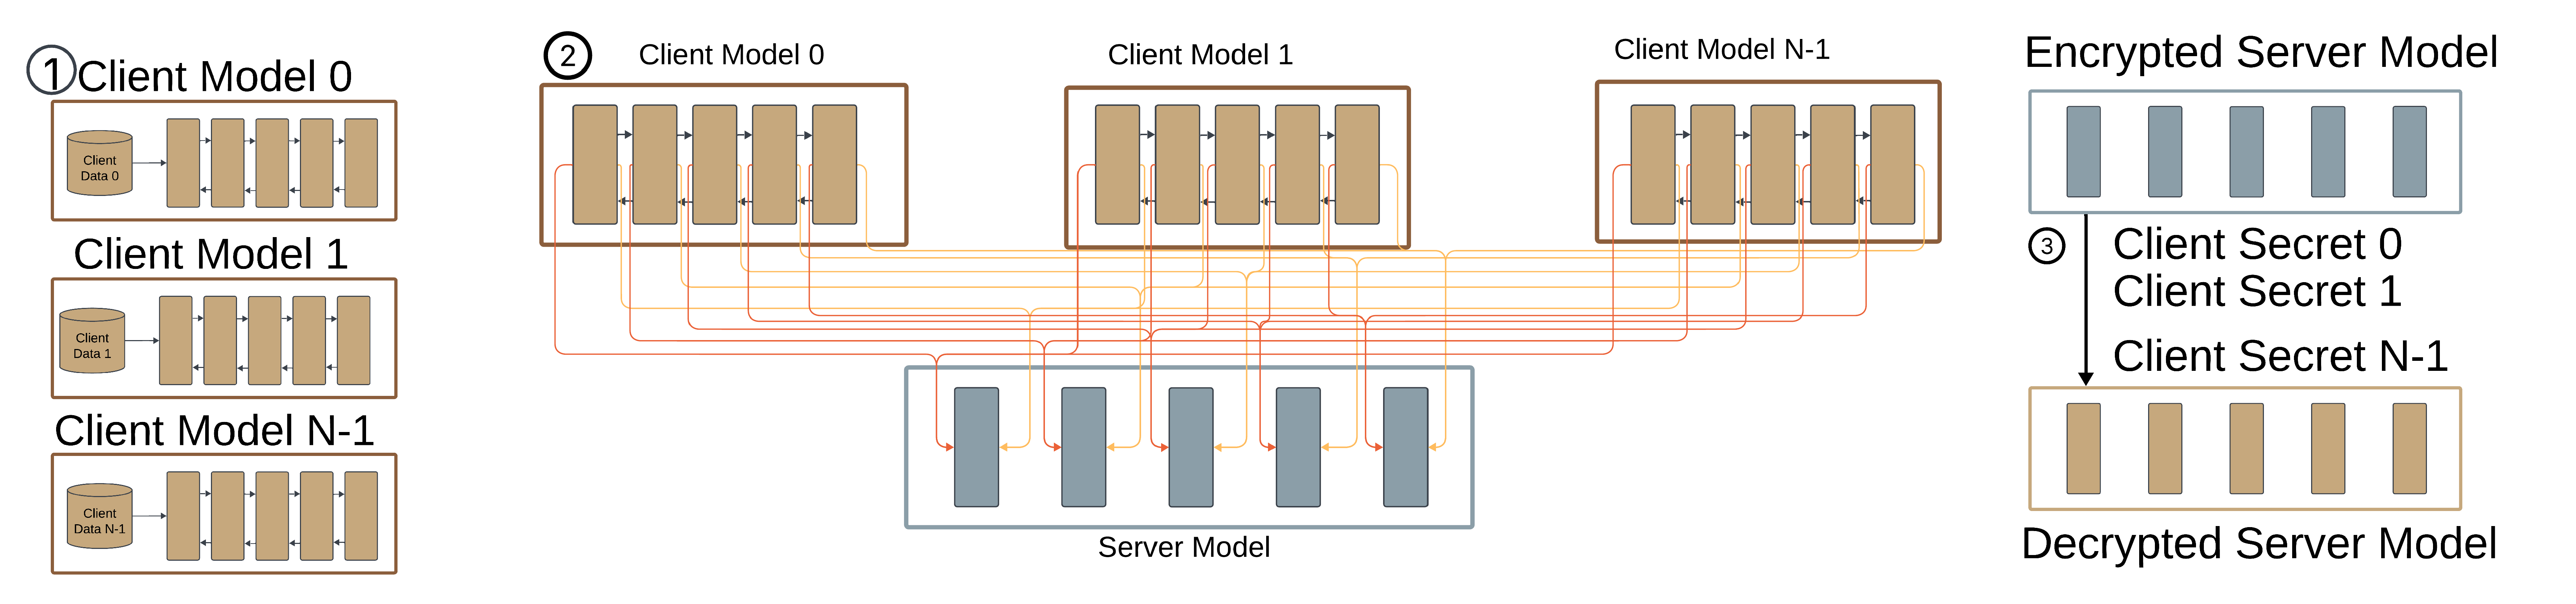
\includegraphics[width=\textwidth]{figures/SysFigureSimple.pdf}

% \caption{Overview of the HE-IFD framework. In Step~1 (Phase~1: Client-Side), each client independently trains a local teacher model on its private dataset, extracts per-block input--output feature pairs, normalises them collaboratively, and encrypts them under CKKS. In Step~2 (Phase~2: Server-Side Distillation), the server acts as a completely blind compute delegate, distilling these encrypted supervision signals block-by-block into an HE-compatible student model (e.g., PolyResNet-18) without ever observing plaintext data, weights, or activations. In Step~3 (Phase~3: Optional Model Release), clients collaboratively perform threshold decryption to release the trained model in plaintext.}

% \label{fig:sys_figure}
% \end{figure*}
 

% \subsection{System Model and Threat Model}
% \label{sec:system_model}

% \par\noindent\textbf{System Model.} We consider a cross-silo federated learning setting with $N$ clients and a central server. Each client $i$ holds a private dataset $\mathcal{D}_i$ that is never shared or transmitted. Clients wish to collaboratively train a shared student model by transferring knowledge from their locally trained teacher models to the server, without exposing their private data, including raw training data and any intermediate logits. Communication between clients and the server is restricted to a single round: each client sends a set of messages derived from its local data and model, after which the server performs all remaining computation independently with no further client interaction. An optional release phase at the end allows clients to collectively obtain the trained model.



% \par\noindent\textbf{Threat Model.} We assume a semi-honest (honest-but-curious) server that follows the protocol faithfully but may attempt to infer private information from everything it observes. All clients are assumed to behave honestly. The adversary's goal is to learn anything about a client's private dataset $\mathcal{D}_i$ or client's local model---including individual samples, label distributions, or model weights---from the messages it receives during training.


% Given this system and threat model, sending plaintext teacher outputs to the server is insufficient: as discussed in Section~\ref{sec:bg_server_inference}, even a single round of plaintext knowledge transfer exposes clients to inference and inversion attacks. We therefore instantiate the knowledge transfer channel using the CKKS homomorphic encryption scheme~\cite{cheon2017ckks}, which allows the server to perform all distillation computation directly on ciphertexts.


% Under the IND-CPA security of CKKS, the server's entire view during training, i.e., encrypted feature pairs, intermediate activations, loss values, gradients, and student weights, is computationally indistinguishable from random. The server operates purely as a blind compute delegate and learns nothing about any client's private data. For additional protection, clients may add calibrated differential privacy noise before encryption, achieving $(\epsilon, \delta)$-differential privacy for the released model; this is optional since the cryptographic guarantee already prevents the server from inspecting any individual contribution during training.



% % \subsubsection{CKKS Depth Budget and Protocol Phases}
% % \label{sec:encryption_params}

% % The CKKS scheme supports approximate arithmetic over real numbers but imposes a finite multiplicative depth budget: each ciphertext--ciphertext multiplication consumes one level, and once exhausted, the ciphertext can no longer be used. HE-IFD manages this budget by design.

% % \textbf{During training}, each block is trained independently with fresh ciphertexts. Since fresh ciphertexts start at full depth, there is no level accumulation across blocks regardless of network depth. The multiplicative depth consumed per block depends only on that block's internal structure: a single PolyBasicBlock containing two degree-2 polynomial activations consumes 2 levels in the forward pass, with additional levels for the backward pass chain rule through the polynomial terms.

% % \textbf{During encrypted inference} (post-deployment), the full student model requires 17 multiplicative levels for a complete forward pass (Section~\ref{sec:ckks_budget}), as the entire network is evaluated as a single encrypted circuit.

% % \textbf{At model release}, if clients elect threshold decryption, the student model weights are decrypted collaboratively and the model can subsequently be used for plaintext inference.


% % \textbf{At model release}, if clients elect threshold decryption, the student model weights are decrypted collaboratively and the model can subsequently be used for plaintext inference.

% \subsection{Overview of HE-IFD}
% \label{sec:overview}

% % Figure~\ref{fig:sys_figure} illustrates the three-phase HE-IFD protocol. In Step~1, each client independently trains a local teacher model on its private data and extracts intermediate feature pairs at each block boundary. In Step~2, clients normalise these features, encrypt them under CKKS, and upload the ciphertexts to the server in a single communication round, which is the only client--server interaction in the entire protocol. In Step~3, the server trains the HE-compatible student model block by block, operating entirely on ciphertexts without ever observing any plaintext data, weights, or activations. At model release, clients may collaboratively perform threshold decryption to obtain the trained student in plaintext; if omitted, the student remains encrypted and can be used directly for encrypted inference.

% HE-IFD proceeds in three phases, illustrated in Figure~\ref{fig:sys_figure} and formalised in Algorithm~\ref{alg:heifd}. In Phase~1, each client independently trains a local teacher model on its private data, extracts intermediate feature pairs at each block boundary, normalises them collaboratively, and uploads the encrypted ciphertexts to the server in a single communication round, which is the only client-to-server interaction in the entire protocol. In Phase~2, the server trains the HE-compatible student model block by block, operating entirely on ciphertexts. This phase proceeds in two stages: Phase~2a, in which each block is trained independently on encrypted teacher features; and Phase~2b, in which the server performs plaintext refinement using trainable bridges to close the train--inference distribution gap, requiring no additional client communication. In the optional Phase~3, clients collaboratively perform threshold decryption to obtain the trained student model in plaintext; if omitted, the student remains encrypted for direct encrypted inference.


% The phases are described in detail below.

% \subsubsection{Phase 1: Client-Side Local Training}
% \label{sec:phase1}

% Each client $i$ trains a local teacher model $T_i$ (e.g., ResNet-18) on their private data $\mathcal{D}_i$ using standard supervised learning. This phase is fully local, ensuring that no data or parameter leaves the client device.

% The server initialises common random weights $\theta_0$ to all clients before local training begins. Each client fine-tunes from $\theta_0$ on their private data. This is standard practice in federated learning and does not constitute a privacy violation: $\theta_0$ is randomly generated and carries no information about any client's data. 
% % In the next section we detail each step in client-side local training.

% % \textbf{Data partitioning.} Data is partitioned across clients using a Dirichlet distribution with concentration parameter $\alpha$, where $\alpha \to 0$ produces extreme non-IID partitions (each client sees few classes) and $\alpha \to \infty$ produces IID partitions. Our experiments evaluate $\alpha \in \{0.1, 0.5, 1.0, 100.0\}$ across $N \in \{1, 2, 4, 8, 16\}$ clients.

% \subsubsection{Phase 2: Per-Block Feature Extraction and Encrypted Upload}
% \label{sec:phase2}

% At a high level, after local training, each client extracts teacher representations at every block boundary, computes normalisation statistics, and uploads encrypted input-output pairs to the server.

% \par\noindent\textbf{Block Boundary Definitions.} We define six blocks matching the teacher and student architectures. Block 0 (stem) takes raw images as input and outputs the result post-conv1, batch normalisation, and ReLU. Block 1 (layer1) takes the stem output and yields features after two BasicBlocks. Blocks 2 through 4 correspond to layers 2 through 4, respectively, incorporating spatial downsampling. Finally, Block 5 (head) processes layer 4 outputs into class logits via average pooling and a fully-connected layer. For each defined block $k$, client $i$ extracts the tuple $(\textbf{x}_k, \textbf{y}_k)$, corresponding respectively to the block's input and output when running the teacher model on local data $\mathcal{D}_i$.

% \par\noindent\textbf{Local Data Protocol.} Each client generates teacher outputs on their \textit{own local training data}~$\mathcal{D}_i$, not on a shared auxiliary dataset. This design has two advantages. First, each teacher evaluates samples from its own training distribution, producing high-confidence supervision signals for the classes it has learned well. A client that specialises in a particular subset of classes provides strong logits and features for those classes, rather than uncertain outputs for classes it has not seen.
% Second, by using each client's data independently without aggregation, the signal from every individual client is preserved at full strength. Under the auxiliary-data protocol (evaluated as a comparison baseline in Section~\ref{sec:experiments}), averaging dilutes the useful signal from specialist clients with weak contributions from clients that have not seen the relevant classes.

% \par\noindent\textbf{Client-Side Collaborative Normalisation.} Before encryption, each client computes per-channel mean and standard deviation over their block-$k$ outputs. 
% For each channel $c$, they normalise their targets to zero mean and unit variance per channel before encryption:
% \begin{equation}
%     \mu_c^{(k,i)} = \mathbb{E}_{x \in \mathcal{D}_i}\!\left[ y_{k,c}(x) \right], \quad
%     \sigma_c^{(k,i)} = \text{Std}_{x \in \mathcal{D}_i}\!\left[ y_{k,c}(x) \right]
%     \label{eq:client_stats}
% \end{equation}
% \begin{equation}
%     \tilde{y}_{k,c} = \frac{y_{k,c} - \mu_c^{(k,i)}}{\sigma_c^{(k,i)}}
%     \label{eq:client_norm}
% \end{equation}
% where $\mu_c^{(k,i)}$ is the per-channel mean, $\sigma_c^{(k,i)}$ is the per-channel standard deviation, $y_{k,c}(x)$ is the $c$-th channel output of block $k$ for input $x$, and $\mathbb{E}$ and $\text{Std}$ denote expectation and standard deviation over the client's local dataset $\mathcal{D}_i$.



% This normalisation is a core component of the protocol, not an optional enhancement. Without it, teachers trained on different data distributions produce features with incompatible magnitude ranges. In our experiments, client-side normalisation eliminates NaN divergence that otherwise occurs at layer3 for $N \geq 4$ clients, and improves student accuracy from ${\sim}$19\% to ${\sim}$37\% at $N{=}4$, $\alpha{=}0.5$ (Section~\ref{sec:experiments}).

% The communication overhead is minimal: $2C$ floating-point values per block per client, where $C$ is the channel count. These statistics can be sent in plaintext (they are aggregate statistics over the client's data, not individual samples) or encrypted if stricter privacy is required.

%  \par\noindent\textbf{Communication Cost.} For each block $k$, client $i$ uploads encrypted input--output pairs for a subset of their local data. As a concrete example, Block~1 (layer1) produces feature maps of shape $64 \times 32 \times 32 = 65{,}536$ elements per sample. With 4096 CKKS slots per ciphertext, a single sample requires 16 ciphertexts per block boundary. Using 20\% of a 5000-sample local dataset (1000 samples), the per-client upload for Block~1 alone amounts to 16{,}000 ciphertexts, each approximately 0.6~MB at $\log N = 13$, giving roughly 9.6~GB per block. This motivates the data-efficiency discussion below.

% % Knowledge distillation is data-efficient: in our experiments, using 20--25\% of each client's local data provides sufficient supervision. The upload is one-shot---no further client interaction is needed during the server-side training loop.
% The upload is one-shot: no further client interaction is needed during the server-side training loop. In our experiments, each client contributes 10\% of their local data as encrypted supervision, which we find sufficient for stable distillation.


% % \subsubsection{Server-Side Block-Level Encrypted Distillation}
% % \label{sec:phase3}
% \subsubsection{Phase 2: Server-Side Distillation}
% \label{sec:phase2_server}

% The server trains the HE-compatible student model block by block. Each block is trained independently with its own fresh ciphertexts, and blocks are composed into the full model after all training is complete.

% \par\noindent\textbf{Block-Level Training.} For each block $k \in \{0, \ldots, 5\}$, the server receives fresh encrypted input--output pairs $\left(\enc{\mathbf{x}_k^{(i,j)}},\, \enc{\tilde{\mathbf{y}}_k^{(i,j)}}\right)$ sourced from every client $i$ and dataset sample $j \in \mathcal{D}_i$. The server conducts sequential multi-teacher training by pooling and shuffling all clients' pairs to bypass loss discontinuities. Gradient steps directly update the encrypted student weights for block $k$. Upon convergence, block $k$'s weights are frozen as permanent ciphertexts, allowing the server to advance to block $k{+}1$ using completely fresh ciphertexts.

% % \textit{No averaging, no aggregation:} Unlike federated averaging approaches, the server does not combine teacher outputs from different clients. Each client's data provides independent gradient steps that accumulate learning into the same set of student block weights. A client with high accuracy on birds contributes strong bird supervision; a client with high accuracy on trucks contributes strong truck supervision. The student learns from both without either signal being diluted.
% Unlike federated averaging approaches, the server does not combine teacher outputs from different clients. Each client's data provides independent gradient steps that accumulate learning into the same set of student block weights. A client with high accuracy on birds contributes strong bird supervision; a client with high accuracy on trucks contributes strong truck supervision. The student learns from both without either signal being diluted.


% % \textit{Fresh ciphertexts per block:} Each block starts training with fresh encrypted input--output pairs from the clients. This is the key design choice that avoids multiplicative level accumulation across blocks. Block $k$'s training consumes a fixed number of CKKS levels determined only by block $k$'s internal structure, regardless of how many blocks precede it.

% Each block starts training with fresh encrypted input--output pairs from the clients. This is the key design choice that avoids CKKS multiplicative budget accumulation across blocks. Block $k$'s training consumes a fixed number of CKKS budget determined only by block $k$'s internal structure, regardless of how many blocks precede it. By arranging the blocks carefully, we avoid costly bootstrapping operations completely.


% \par\noindent\textbf{Train--Inference Distribution Alignment.} For block $k > 0$, the input to block $k$ at inference is the output of the student's frozen prefix (blocks $0 \to k{-}1$). If block $k$ is instead trained on teacher-produced inputs, which we call \textit{teacher-input training}, a distribution gap arises: the features the teacher's prefix produces differ systematically from those the student's prefix produces, since the student uses polynomial activations rather than ReLU. If not addressed, this mismatch propagates through all subsequent blocks and causes the composed model to collapse toward random accuracy.

% % \textit{The ideal but communication-expensive fix.} The cleanest solution is \textit{student-input training}: after block $k{-}1$ is frozen, the server publishes its weights to all clients; each client runs the frozen student prefix locally and uploads fresh ciphertexts of the resulting student-produced inputs for block $k$. This completely eliminates the distribution gap but requires one additional client--server round per block---$K$ extra rounds for a $K$-block model---which conflicts with our one-shot communication objective.

% The cleanest solution is \textit{student-input training}: after block $k{-}1$ is frozen, the server publishes its weights to all clients; each client runs the frozen student prefix locally and uploads fresh ciphertexts of the resulting student-produced inputs for block $k$. This completely eliminates the distribution gap but requires one additional client--server round per block---$K$ extra rounds for a $K$-block model---which conflicts with our one-shot communication objective.


% Our approach is a one-shot upload with teacher-input and server-side alignment. We retain the one-shot upload property by using teacher-input training throughout Phase~2a but compensating for the distribution gap through two complementary mechanisms.

% % \textit{(i) Trainable bridges.} Each block group is followed by a \textit{TrainableBridge} module: a per-channel affine transform $\mathbf{b}_k(\mathbf{h}) = \boldsymbol{\gamma}_k \odot \mathbf{h} + \boldsymbol{\beta}_k$ with learned scale $\boldsymbol{\gamma}_k$ and bias $\boldsymbol{\beta}_k$. After Phase~2a, the server initialises each bridge to minimise the distribution shift from teacher-prefix to student-prefix features using the uploaded feature statistics:
% \par\noindent\textbf{Phase~2a: Encrypted Block-Level Training.} Each block group is followed by a \textit{TrainableBridge} module: a per-channel affine transform $\mathbf{b}_k(\mathbf{h}) = \boldsymbol{\gamma}_k \odot \mathbf{h} + \boldsymbol{\beta}_k$ with learned scale $\boldsymbol{\gamma}_k$ and bias $\boldsymbol{\beta}_k$. After Phase~2a, the server initialises each bridge to minimise the distribution shift from teacher-prefix to student-prefix features using the uploaded feature statistics:

% \begin{equation}
%     \boldsymbol{\gamma}_k \leftarrow \frac{\sigma\!\left[f^T_k(\mathbf{x})\right]}{\sigma\!\left[S_{0:k}(\mathbf{x})\right]}, \qquad
%     \boldsymbol{\beta}_k \leftarrow \mu\!\left[f^T_k(\mathbf{x})\right] - \boldsymbol{\gamma}_k \odot \mu\!\left[S_{0:k}(\mathbf{x})\right],
%     \label{eq:bridge_init}
% \end{equation}
% where $f^T_k$ denotes the teacher's block-$k$ output and $S_{0:k}$ the student chain through block $k$. This initialises each bridge as a near-identity transform (scale $\approx 1$, bias $\approx 0$) that aligns the student's feature distribution to the teacher's at each stage, preventing the cascade collapse that otherwise occurs in teacher-input training.

% % \textit{(ii) Server-side sequential refinement (Phase~2b).} After bridge initialisation, the server runs additional refinement rounds using the already-uploaded plaintext features. In each round, blocks are refined sequentially: block $k$ is trained on the actual output of the student's refined prefix (blocks $0 \to k{-}1$), with the teacher's block-$k$ output as the target. This is equivalent to student-input training, but executed entirely server-side on plaintext features---no additional client communication is required. Bridge parameters are co-trained alongside block weights during refinement.

% \par\noindent\textbf{Phase~2b: Server-Side Plaintext Refinement.} After bridge initialisation, the server runs additional refinement rounds using the already-uploaded plaintext features. In each round, blocks are refined sequentially: block $k$ is trained on the actual output of the student's refined prefix (blocks $0 \to k{-}1$), with the teacher's block-$k$ output as the target. This is equivalent to student-input training, but executed entirely server-side on plaintext features---no additional client communication is required. Bridge parameters are co-trained alongside block weights during refinement.

% The cryptographic cost analysis of both phases is provided in Section~\ref{sec:encryption_params}.



% \par\noindent\textbf{Loss Function.} Each block is trained with a magnitude-regularised normalised MSE loss.

% Student and teacher features are normalised per channel to zero mean and unit variance before computing MSE:
% \begin{equation}
%     \mathcal{L}_{\text{NormMSE}} = \frac{1}{C} \sum_{c=1}^{C} \text{MSE}\!\left(\frac{\hat{f}_c - \mu_{\hat{f}_c}}{\sigma_{\hat{f}_c}},\; \frac{\tilde{f}_c - \mu_{\tilde{f}_c}}{\sigma_{\tilde{f}_c}}\right)
%     \label{eq:normmse}
% \end{equation}
% where $\hat{f}_c$ and $\tilde{f}_c$ are the student prediction and normalised teacher target for channel $c$. This scale-invariant loss handles the distributional mismatch between PolyAct student activations (signed, potentially large) and ReLU teacher activations (non-negative, bounded).

% \par\noindent\textbf{Magnitude regularisation.} NormMSE alone is scale-invariant and permits the student to grow magnitudes without penalty. Since subsequent frozen polynomial blocks amplify any scale drift, we add a log-ratio penalty:
% \begin{equation}
%     \mathcal{L}_{\text{MagReg}} = \mathcal{L}_{\text{NormMSE}} + \lambda \cdot \frac{1}{C} \sum_{c=1}^{C} \left(\log \frac{\sigma_{\hat{f}_c}}{\sigma_{\tilde{f}_c}}\right)^{\!2}
%     \label{eq:magreg}
% \end{equation}
% The log-ratio form is symmetric (penalises student magnitudes that are too large or too small equally) and scale-free (proportional to the multiplicative mismatch). The regularisation weight $\lambda$ scales with block depth: $\lambda = 2$ for early blocks, increasing to $\lambda = 6$ for deeper blocks where magnitude accumulation from the frozen chain is more severe.

% \par\noindent\textbf{MSE on logits.} For the head block (block 5), which outputs class logits, we use plain MSE without normalisation or magnitude regularisation, since logits are low-dimensional and do not exhibit the spatial channel structure of intermediate features.

% We use MSE rather than KL divergence because softmax is not a polynomial operation and cannot be evaluated under CKKS encryption. MSE on raw logits is HE-compatible: the squaring operation requires one ciphertext--ciphertext multiplication (1 CKKS level), and the remaining subtraction and averaging are level-free.

% % \subsection{Protocol Summary}
% % \label{sec:algorithm}

% %     The HE-IFD protocol proceeds in three phases. In Phase~1 (local), each client independently trains a teacher model and extracts per-block input--output feature pairs from its private data. In Phase~2 (single upload), clients normalise their features using collaborative per-channel statistics, encrypt them under the CKKS scheme, and transmit the ciphertexts to the server in a single communication round. In Phase~3 (server-side distillation), the server trains the HE-compatible PolyResNet-18 student block by block, where each block receives fresh ciphertexts from all clients and is optimised via encrypted gradient descent before being frozen. An optional Phase~4 allows clients to collaboratively perform threshold decryption to release the trained model in plaintext. Algorithm~\ref{alg:heifd} formalises this procedure.


% % Before describing Phase~3, we summarise how HE-IFD manages the CKKS multiplicative depth budget across the protocol phases.

% \subsubsection{CKKS Depth Budget and Protocol Phases}
% \label{sec:encryption_params}

% The CKKS scheme supports approximate arithmetic over real numbers but imposes a finite multiplicative depth budget: each ciphertext--ciphertext multiplication consumes one level, and once exhausted, the ciphertext can no longer be used. HE-IFD manages this budget by design.

% \textbf{During training}, each block is trained independently with fresh ciphertexts. Since fresh ciphertexts start at full depth, there is no level accumulation across blocks regardless of network depth. The multiplicative depth consumed per block depends only on that block's internal structure: a single PolyBasicBlock (defined in Section~\ref{sec:polybasicblock}) containing two degree-2 polynomial activations consumes 2 levels in the forward pass, with additional levels for the backward pass chain rule through the polynomial terms.

% \textbf{During encrypted inference} (post-deployment), the full student model requires 17 multiplicative levels for a complete forward pass (Section~\ref{sec:ckks_budget}), as the entire network is evaluated as a single encrypted circuit.

% \textbf{At model release}, if clients elect threshold decryption, the student model weights are decrypted collaboratively and the model can subsequently be used for plaintext inference.

% \subsubsection{Phase~3 (Optional): Model Release}
% \label{sec:phase3}

% After server-side distillation is complete, the trained student model weights remain encrypted as ciphertexts on the server. Clients may collaboratively perform threshold decryption to obtain the student model in plaintext, after which it can be deployed for standard inference. If this phase is omitted, the student remains encrypted and can be used directly for encrypted inference without further client involvement.
% \par\noindent\textbf{CKKS depth constraint.} Teacher-input Phase~2a trains each block in isolation: block $k$ consumes only the CKKS levels determined by its own internal operations, independent of model depth. No level accumulation occurs across blocks, and no bootstrapping is needed during Phase~2a. Phase~2b refinement operates entirely on plaintext features already held by the server and therefore incurs no CKKS cost. At inference, the full student chain with bridges consumes levels sequentially; this depth budget is analysed in Section~\ref{sec:ckks_budget}.

% % \subsection{Details of HE-IFD}
% % \label{sec:details}
% % \hl{remove?}
% \begin{algorithm}[h!]
% \small
% \caption{HE-IFD: HE-Based Intermediate Feature Distillation}
% \label{alg:heifd}
% \begin{algorithmic}[1]
% \REQUIRE $N$ clients with private datasets $\mathcal{D}_1, \ldots, \mathcal{D}_N$; HE-compatible student architecture $S$ with $K{+}1$ blocks
% \ENSURE Trained student model $S$ (encrypted or decrypted)

% \STATE \textbf{--- Phase 1: Client-Side (parallel, local) ---}
% \FOR{each client $i = 1, \ldots, N$ \textbf{in parallel}}
%     \STATE Train teacher $T_i$ on $\mathcal{D}_i$ via standard SGD
%     \FOR{each block $k = 0, \ldots, K$}
%         \STATE Extract input--output pairs $(\mathbf{x}_k^{(i,j)}, \mathbf{y}_k^{(i,j)})$ by running $T_i$ on $\mathcal{D}_i$
%         \STATE Compute per-channel statistics: $\mu_c^{(k,i)}, \sigma_c^{(k,i)}$ over $\mathbf{y}_k$ \hfill\COMMENT{Eq.~\ref{eq:client_stats}}
%         \STATE Normalise targets: $\tilde{\mathbf{y}}_k^{(i,j)} \leftarrow (\mathbf{y}_k^{(i,j)} - \mu) / \sigma$ \hfill\COMMENT{Eq.~\ref{eq:client_norm}}
%     \ENDFOR
%     \STATE Encrypt all pairs under CKKS; upload $\{\enc{\mathbf{x}_k^{(i,j)}}, \enc{\tilde{\mathbf{y}}_k^{(i,j)}}\}$ to server
% \ENDFOR

% \STATE
% % \STATE \textbf{--- Phase 2: Server-Side Block Distillation ---}
% \STATE \textbf{--- Phase 2a: Server-Side Encrypted Distillation ---}

% \STATE Initialise student $S$ with near-linear PolyAct ($a{=}0.3, b{=}0.7, c{=}0$)
% \FOR{block $k = 0, \ldots, K$}
%     \STATE Pool encrypted pairs from all $N$ clients for block $k$; shuffle
%     \STATE Set $\lambda_k \leftarrow \lambda_{\text{base}} \cdot (1 + 2 \cdot k/K)$ \hfill\COMMENT{deeper blocks: stronger MagReg}
%     \STATE Set $\eta_k \leftarrow \eta_{\text{base}} \cdot (1 - 0.8 \cdot k/K)$ \hfill\COMMENT{deeper blocks: lower LR}
%     \FOR{epoch $= 1, \ldots, E$}
%         \FOR{each mini-batch $(\enc{\mathbf{x}}, \enc{\tilde{\mathbf{y}}_k})$}
%             \IF{$k = 0$}
%                 \STATE $\mathbf{h} \leftarrow \enc{\mathbf{x}}$ \hfill\COMMENT{raw image input}
%             \ELSE
%                 \STATE $\mathbf{h} \leftarrow \enc{\mathbf{x}_k}$ \hfill\COMMENT{teacher-produced input, uploaded by clients}
%             \ENDIF
%             \STATE $\hat{\mathbf{y}} \leftarrow S_{\text{block}[k]}(\mathbf{h})$ \hfill\COMMENT{current block forward}
%             \IF{$k < K$}
%                 \STATE $\mathcal{L} \leftarrow \mathcal{L}_{\text{NormMSE}}(\hat{\mathbf{y}}, \enc{\tilde{\mathbf{y}}_k}) + \lambda_k \cdot \mathcal{L}_{\text{MagReg}}(\hat{\mathbf{y}}, \enc{\tilde{\mathbf{y}}_k})$ \hfill\COMMENT{Eq.~\ref{eq:magreg}}
%             \ELSE
%                 \STATE $\mathcal{L} \leftarrow \text{MSE}(\hat{\mathbf{y}}, \enc{\tilde{\mathbf{y}}_k})$ \hfill\COMMENT{logit block}
%             \ENDIF
%             \STATE Update $S_{\text{block}[k]}$ via encrypted gradient descent with learning rate $\eta_k$
%         \ENDFOR
%     \ENDFOR
%     \STATE Freeze $S_{\text{block}[k]}$
% \ENDFOR

% \STATE
% \STATE \textbf{--- Phase 2b: Server-Side Plaintext Refinement ---}
% \STATE Initialise bridges; refine all blocks sequentially on uploaded plaintext features \hfill\COMMENT{Section~\ref{sec:phase2_server}}

% \STATE
% \STATE \textbf{--- Phase 3 (optional): Model Release ---}
% \STATE Clients collaboratively perform threshold decryption to obtain $S$ in plaintext
% \end{algorithmic}
% \end{algorithm}


% \subsection{HE-Compatible Student Architecture}
% \label{sec:architecture}

% The student is a PolyResNet-18 which is structurally identical to the teacher ResNet-18 but with all HE-incompatible operations replaced. This structural correspondence enables block-level feature matching between teacher and student.

% \subsubsection{Component Replacements}
% Here, we explain how we enable efficient execution of several functions in HE-IFD. 
% \par\noindent\textbf{ReLU $\to$ PolyAct.} ReLU is a function ($\max(0, x)$) with no efficient polynomial representation under CKKS. We replace it with a learnable degree-2 polynomial:
% \begin{equation}
%     \text{PolyAct}(x) = ax^2 + bx + c
%     \label{eq:polyact}
% \end{equation}
% % initialised at $a = 0.3$, $b = 0.7$, $c = 0$, so that the initial behaviour is approximately linear ($\text{PolyAct}(x) \approx 0.7x$ for small $x$). The coefficients are learnable and adapt during training; after training, they are frozen as plaintext constants. 

% initialised at $a = 0.3$, $b = 0.7$, $c = 0$, so that for normalised inputs ($|x| \leq 1$) the activation behaves approximately linearly ($\text{PolyAct}(x) \approx 0.7x$), avoiding early magnitude divergence from the quadratic term. This near-linear initialisation strategy is consistent with prior work on stable polynomial-activation training~\cite{baruch2022methodology, garimella2021sisyphus}; the specific values were validated empirically. The coefficients are learnable and adapt during training and after training, they are frozen as plaintext constants.


% Under CKKS, $x^2$ is one ciphertext--ciphertext multiplication (1 multiplicative level). The remaining terms ($ax^2, bx, c$) involve only plaintext--ciphertext operations (0 levels). Thus, the total cost is 1 multiplicative level per activation. 

% \par\noindent\textbf{BatchNorm $\to$ ChannelScale.} Batch normalisation computes a normalised output $\hat{x} = (x - \mu)/\sigma$ followed by a learnable affine transform. Under CKKS, the division $x/\sigma$ has no direct equivalent and must be approximated via iterative methods such as Goldschmidt's algorithm, which requires ${\sim}$10 multiplicative levels per invocation — far too expensive for a deep network. Since batch statistics are fixed after training, the normalisation can be folded into the affine parameters, leaving only the learnable scale and bias. We therefore replace BatchNorm with ChannelScale, a per-channel affine transform that is equivalent to BatchNorm at inference but costs zero multiplicative levels. 
% % We replace it with a per-channel affine transform:
% \begin{equation}
%     \text{ChannelScale}(x) = \gamma \odot x + \beta
%     \label{eq:channelscale}
% \end{equation}
% with learnable $\gamma$ (initialised to 1) and $\beta$ (initialised to 0). Since both are known plaintext at inference, this costs 0 multiplicative levels.

% \par\noindent\textbf{MaxPool $\to$ identity.} Max pooling is a comparison operation that requires non-polynomial approximations (e.g., iterative sign functions) with prohibitive multiplicative depth under CKKS. For CIFAR-10 (32$\times$32 input), the initial max pool in standard ResNet-18 was not adopted due to this high computational demand and is replaced by an identity operation. Spatial downsampling is handled by stride-2 convolutions in layers 2--4.

% \subsubsection{PolyBasicBlock Structure}\label{sec:polybasicblock}

% % Each PolyBasicBlockV2 follows the dataflow:
% Each PolyBasicBlock, the residual building block of PolyResNet-18, replacing the standard BasicBlock with HE-compatible operations, follows the dataflow:

% \begin{equation}
%     x \xrightarrow{\text{conv}_1} \xrightarrow{\text{CS}_1} \xrightarrow{\text{PolyAct}_1} \xrightarrow{\text{conv}_2} \xrightarrow{\text{CS}_2} \xrightarrow{+\,\text{identity}} \xrightarrow{\text{PolyAct}_2} y
% \end{equation}
% where conv denotes a convolution layer, CS denotes ChannelScale, PolyAct is the polynomial activation defined in Eq.~\ref{eq:polyact}, and $+\,\text{identity}$ is the residual addition.

% Convolutions, ChannelScale, and the residual addition consume 0 levels. The two PolyAct invocations consume 1 level each, for a total of 2 multiplicative levels per block.

% \subsubsection{Multiplicative Depth of CKKS Inference}
% \label{sec:ckks_budget}

% \begin{table}[h]
% \centering
% \caption{CKKS multiplicative levels for PolyResNet-18 encrypted inference}
% \label{tab:ckks_levels}
% \begin{tabular}{l|c|c|c}
% \hline
% \textbf{Component} & \textbf{Levels/Block} & \textbf{Blocks} & \textbf{Total} \\
% \hline
% Stem (conv $+$ CS $+$ PolyAct) & 1 & 1 & 1 \\
% Layer 1 (2 PolyBasicBlocks) & 2 & 2 & 4 \\
% Layer 2 & 2 & 2 & 4 \\
% Layer 3 & 2 & 2 & 4 \\
% Layer 4 & 2 & 2 & 4 \\
% AvgPool $+$ FC & 0 & --- & 0 \\
% \hline
% \textbf{Total} & & & \textbf{17} \\
% \hline
% \end{tabular}
% \end{table}

% % At inference, model weights are frozen plaintext constants. All operations involving weights (convolution, ChannelScale, FC) are plaintext--ciphertext and consume 0 levels. Only PolyAct's $x^2$ term consumes one multiplicative level per execution; all other operations are level-free.

% % During \textit{encrypted training}, server weights become ciphertext after the first gradient update involving encrypted targets. Operations previously marked PT$\times$CT become CT$\times$CT (1 additional level each). However, because each block trains independently with fresh ciphertexts, this increased cost is confined to the current block's depth budget and does not accumulate across the full network.

% \subsubsection{Total Number of CKKS Levels per Operation}

% Table~\ref{tab:he_ops} shows that at inference, only PolyAct consumes a multiplicative level (1 per invocation), since all other operations either involve plaintext weights (PT$\times$CT, 0 levels) or are level-free additions. During training, weights become ciphertext after the first gradient update, adding 1 level to convolution, ChannelScale, and the FC layer; however, since each block trains independently with fresh ciphertexts, this cost is confined to a single block and never accumulates across the network.

% \begin{table}[h]
% \centering
% \caption{CKKS costs per operation. At inference, weights are plaintext (PT) and activations are ciphertext (CT). During training, weights become CT after the first encrypted gradient update.}
% \label{tab:he_ops}
% \begin{tabular}{l|l|c|c}
% \hline
% \textbf{Operation} & \textbf{Inference} & \textbf{Inf.\ Levels} & \textbf{Train Levels} \\
% \hline
% Convolution & PT$\times$CT & 0 & 1 \\
% ChannelScale & PT$\times$CT & 0 & 1 \\
% PolyAct ($ax^2{+}bx{+}c$) & CT$\times$CT & 1 & 1 \\
% Residual add & CT$+$CT & 0 & 0 \\
% Average pooling & $\Sigma$CT $\times$ PT & 0 & 0 \\
% FC layer & PT$\times$CT & 0 & 1 \\
% \hline
% \end{tabular}
% \end{table}

% \subsection{Training Stability}
% \label{sec:stability}

% % Polynomial activations introduce unique training challenges that require multiple interlocking stability mechanisms.

% Polynomial activations introduce unique training challenges. We describe the main source of instability below and then present the interlocking mechanisms we deploy to address it.


% \subsubsection{Magnitude Accumulation}
% The quadratic term in PolyAct amplifies activation magnitudes at every composition. With $\text{PolyAct}(x) = 0.3x^2 + 0.7x$, an input of magnitude 5 produces output ${\sim}$11; a further composition gives ${\sim}$44. After 5 compositions (typical by layer3), magnitudes can reach $10^4$, causing NaN divergence. This problem is exacerbated under multi-client settings ($N \geq 4$), where heterogeneous client distributions increase feature variance through the frozen chain.

% The stability mechanisms described below address this problem directly.


% \subsubsection{Stability Mechanisms}

% % We deploy several interlocking mechanisms to counter instability. Client-side normalisation (Eq.~\ref{eq:client_norm}) bounds target ranges before encryption to avert cross-client magnitude mismatch. A magnitude-regularised loss (Eq.~\ref{eq:magreg}) constrains student scales to teacher targets, curtailing unbounded growth through frozen polynomial sequences. ChannelScale contributes per-channel affine capacity, substituting the variance normalisation lost by omitting batch normalisation. Strict gradient clipping ($\text{max\_norm} = 1.0$) inherently controls gradient explosion originating from quadratic terms. Crucially, student-input training (Section~\ref{sec:phase3}) subjects each block to the accurate inference-time distribution, precluding the catastrophic accuracy collapse characteristic of teacher-input paradigms. Furthermore, block-independent training employing fresh ciphertexts suppresses CKKS level accumulation, ensuring pristine numerical starts. Finally, deeper blocks incorporate strict learning rate scaling (operating down to $0.2\times$ base rates for layer 4) to mitigate sensitivity to accumulated perturbations from extended frozen prefix chains. 

% We deploy the following mechanisms to address the instability described above. Client-side normalisation (Eq.~\ref{eq:client_norm}) ensures that teacher features from different clients have compatible magnitude ranges before encryption. The magnitude-regularised loss (Eq.~\ref{eq:magreg}) penalises the student when its output scale drifts from the teacher target, preventing unbounded growth through the frozen polynomial chain. ChannelScale provides per-channel affine capacity at each block, compensating for the absence of batch normalisation. Gradient clipping (max\_norm$=$1.0) prevents large gradient steps from the quadratic term. Student-input training (Section~\ref{sec:phase2_server}) ensures each block is trained on the same input distribution it will receive at inference, avoiding the collapse observed in teacher-input training. Finally, learning rates are scaled down for deeper blocks (to $0.2\times$ the base rate at layer~4) to account for the larger input variance accumulated through the frozen prefix chain.


% Our ablation study (Section~\ref{sec:ablation}) quantifies the accuracy impact of removing each mechanism individually. In particular, removing client-side normalisation causes NaN divergence for $N \geq 4$; removing the magnitude regularisation penalty degrades accuracy by ${\sim}$18\%; and replacing student-input with teacher-input training reduces accuracy from ${\sim}$71\% to ${\sim}$12\%.

% \subsection{Privacy Analysis}
% \label{sec:privacy_proof}

% %We provide a formal privacy argument for the HE-IFD protocol. 
% We assume the server is "honest-but-curious": it follows the protocol but may try to learn client data from what it sees. We assume all $N$ clients are honest. During training, the server only sees CKKS-encrypted input--output pairs, basic metadata such as the number of clients and tensor sizes, and optional plaintext normalisation statistics. Everything else---such as student weights, activations, losses, and gradients---is computed homomorphically and remains fully encrypted.

% Under the Ring Learning with Errors (RLWE) assumption (with security parameter $\lambda \geq 128$), our protocol guarantees that the server learns no private information about individual client data during training. This relies on the IND-CPA security of the CKKS scheme~\cite{cheon2017ckks}, which means encrypted data cannot be distinguished from random noise. Because all homomorphic operations simply map ciphertexts to other ciphertexts, every intermediate calculation stays secure. As a result, the server's entire view of the training process can be simulated using only public parameters and metadata, proving no data is leaked. If clients choose to send their normalisation statistics in plaintext, these are aggregate quantities computed over the full local dataset and carry non-critical information about any individual sample. For maximum security, these statistics can also be encrypted. Thus, privacy against server is achieved.

% If clients choose to decrypt the trained model for release, the resulting plaintext model has the same risk of membership inference attacks by clients~\cite{shokri2017membership, carlini2022membership} as any standard machine learning model. Homomorphic encryption prevents data leakage during training without adding noise or limiting the number of training steps. In contrast, differential privacy (DP) adds noise to protect the final model, which lowers accuracy and limits how much training can be done. However, our protocol easily supports both: clients can add DP noise to their data before encrypting it. This provides a formal $(\epsilon, \delta)$-DP for the final decrypted model without changing how the encrypted training works.